% THIS IS SIGPROC-SP.TEX - VERSION 3.1
% WORKS WITH V3.2SP OF ACM_PROC_ARTICLE-SP.CLS
% APRIL 2009
%
% ----------------------------------------------------------------------------------------------------------------
% This .tex file (and associated .cls V3.2SP) *DOES NOT* produce:
%       1) The Permission Statement
%       2) The Conference (location) Info information
%       3) The Copyright Line with ACM data
%       4) Page numbering
% ---------------------------------------------------------------------------------------------------------------
% For tracking purposes - this is V3.1SP - APRIL 2009

\documentclass{acm_proc_article-sp}
\usepackage{graphicx}
\usepackage{hyperref}

\makeatletter
\def\@copyrightspace{\relax}
\makeatother

\begin{document}

\title{Copy and Paste Habits and Improvements for the Everyday Programmer}
\subtitle{February 1 Deliverable\thanks{This report is Group G's first project deliverable for CSC 510 in the Spring of 2016 taught by Dr. T. Menzies at North Carolina State University.}}

\numberofauthors{4} 
\author{
\alignauthor
Brian Clee\\
       %\affaddr{NC State University}\\
       %\affaddr{Address One}\\
       \email{bpclee@ncsu.edu}
\alignauthor
Effat Farhana\\
       %\affaddr{NC State University}\\
       %\affaddr{Address Two}\\
       \email{efarhan@ncsu.edu}
\and % go to new row
\alignauthor
Arjun Madan\\
       %\affaddr{NC State University}\\
       %\affaddr{Address Three}\\
       \email{amadan2@ncsu.edu}
\alignauthor
Ran Tan\\
       %\affaddr{NC State University}\\
       %\affaddr{Address Four}\\
       \email{rtan2@ncsu.edu}
}

\date{1 February 2016}
\maketitle

\begin{abstract}
Computer programmers rely on a myriad of tools and production environments in order to produce quality software in a productive manner. Of these tools the simple copy and paste command is used frequently by programmers to save time. In this paper we examine the behavioral motivations as to why programmers make use of the copy and paste command, as well as when and how they actually use it. As well, we investigate the problems that can arise from using this command in the form of code clones and duplications, and their implications. Finally we propose a project wherein we will be building a fully feature Eclipse IDE plug-in, Clipit, which will give Java programmers a visual clipboard manager that enhances their productivity when copying and pasting, and alleviates the problems caused by using this common command.
\end{abstract}

%see http://www.acm.org/sigs/publications/sigguide-v2.2sp section 2.3.2
% A category with the (minimum) three required fields
\category{D.2.2}{Software Engineering}{Design Tools and Techniques}[Modules and interfaces, programmer workbench, user interfaces]
%A category including the fourth, optional field follows...
\category{D.2.3}{Software Engineering}{Coding Tools and Techniques}[Program Editors]

% see http://www.acm.org/sigs/publications/sigguide-v2.2sp section 2.3.3
\terms{Human Factors, Management, Performance, Theory}

\keywords{Code cloning, code duplication, copy and pasting, eclipse plug-ins, programmer habits, programmer productivity}

\section{Introduction}
One of the most common operations computer users apply in their daily computer use is copy and paste. An incredibly simple to understand tool, copy and paste allows users to take information from one location, briefly store it, and then leave that information elsewhere. This simple tool is commonplace for computer users, and it is especially useful to computer programmers.

In the field of computer programming, users frequently make use of the copy and past operation for a myriad of reasons. For one, it is essential in the practice of relocating, regrouping, or reorganizing code from one place to another. Along these lines programmers also use the command in the act of reordering parts of their code, rather than rewriting. Finally, perhaps the most common use of the copy and paste command is when a programmer copies a block of code, either from inside sources within their existing code base or outside it, to use as a structural template ~\cite{ooplCP}.

However, while there is much to be gained from the copy and paste operation for programmers, it is also important to realize that despite the operation's convenience and simplicity, the act of copying and pasting introduces a variety of errors. In one study analyzing programmer habits, it was found that copying and pasting can introduce errors by pasting incomplete copies, and failing to update their context. In this study they found that these sorts of errors actually reduced productivity as a whole for the programmer by delaying development in the long run ~\cite{maintenenceStudy}

Yet despite the apparent errors that can be introduced by copying and pasting, programmers still make use of the operation in their core work-flow. In another study done it was found that on average every programmer copy and pastes 16 times while programming ~\cite{ooplCP}. Clearly this command has become part of programming vernacular despite the problems it can cause.

In this paper we investigate the copy and paste command as used in software engineering in greater detail. In particular we present a literature review on the topic as it has been investigated in numerous studies and research experiments. We look at the user patterns and behavioral components that go into using this command, as well as the command itself in practice. We also look at heavier theoretical applications to copying and pasting such as code cloning and pattern detection. Ultimately though, we use this research to show that there is untapped potential in the copy and paste command for programmers, which can be addressed by a fully featured clipboard manager plug-in for the Eclipse IDE, similar to one described in ~\cite{ooplCP}.

\section{User Patterns and Behavior}
In this section we discuss in further detail why and how programmers use the copy and paste command in their daily work-flow. As discussed in the introduction, this command is actually used quite frequently, as one IBM study has shown it is used on average 16 times an hour by professional programmers. Specifically, this study followed nine IBM Watson researches for 60 hours while they coded in Java in their natural working environment. Essentially the researches broke this group of nine programmers into two case studies, the first of which involved direct observations with questions throughout ten hours of coding. While the second of which involved using a background logger and replayer system integrated into the participants' machines which allowed for 50 hours of observation yet less interviews. This study is described in figure  \ref{fig:oopl}~\cite{ooplCP}, and the report surrounding this study has been widely cited 240 times since 2004, we will reference it frequently throughout our report.

 \begin{figure}[h]
 \centering
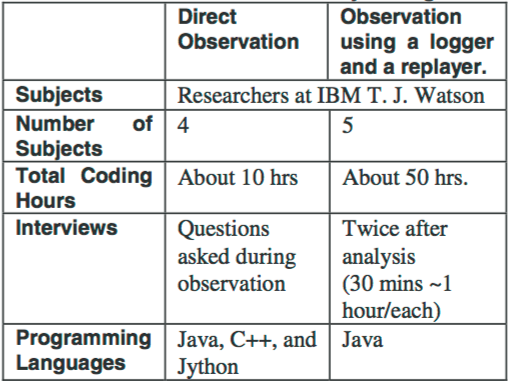
\includegraphics[width=8cm]{ooplStudy}
\caption{Description of Study Environment}
    \label{fig:oopl}
\end{figure}

According to this IBM study, they observed that 74\% of all copy and paste instances copied text less than a single line. These cases would be simple copies like copying a variable name, a type or method declaration, and in these cases the command was most likely used for the sake of saving typing time. Of the remaining copies, however, they found that these were instances of copying blocks of code. Specifically in these cases the use of the copy and paste command created code duplicates and heavily reflected in the resulting structure of the code base ~\cite{ooplCP}.

The reason these structural code duplicates are important, is because there is an entire field of research focused on the errors that occur because of code duplicates ~\cite{devWorkHabits}. Even though according to one study these types of artifacts are only created roughly 25\% of the time, if you multiply that by the average 16 copy and paste instances per hour that means that the average professional programmer creates four non-trivial copy and paste dependencies per hour ~\cite{ooplCP}. 

But what exactly do these non-trivial dependencies look like? To answer this we turn to a Microsoft study which consisted of thoroughly surveying and interviewing professional programmers who worked at Microsoft Corporation. This study is quite influential and has been cited 367 times since 2006, for the most part though it's influence is felt in other areas programmer habit study, though they specifically spent a section of their report discussing copy and paste habits. They conducted their study by creating a participant pool of 6000 programmers at Microsoft Corporation, and sending out two different surveys to subsets of size 200 from the participant pool. In both cases the subsets were asked roughly 200 questions and participation was nearly complete. Finally, after conducting both surveys 11 individual programmers were individually interviewed ~\cite{devWorkHabits}. 

In the results of their interviews these researches found that could create a taxonomy of categories of code duplication, and further detail the frequency of each category and importance of the problem ~\cite{devWorkHabits}. Some of these categories are unrelated to our concerns on copy and paste habits, yet three are particularly relevant. 

The first involves 'example clones' which refers to code that is copied from an outside source and is used as an example, or a template, for use in a new context. These clones were actually the most studied, and the researchers found that it is difficult to say one way or another if the clones would be better off factored into a new abstraction. 

The second category is 'scattered clones', or logical clones, and these are similar to the majority of copy and paste instances discussed earlier. For the most part these clones are simply the copy and paste of variable names, method headers, etc., and due to their nature they tend to propagate themselves throughout a code base. Because of this duplicitous nature, these duplicates can be hard to manage en masse, and multiple interviewees reported that when dealing with changing a root duplicate in these cases they would often "hope for the best" and hope that testers found any other necessary changes.

Finally, the third relevant category for copy and pasting deals with 'fork clones'. These types of clones occur when a developer 'forks' another code base by literally copying the entire thing to start new development on. In the production environment this can occur when a team needs to use code that another team isn't ready to ship, so they are forced to create a full copy of it and start tailoring it to their needs. In nearly every interview the subjects reported that when possible it is best to avoid these types of clones, unless the only alternative is to implement the functionality from scratch. When these are necessary, a higher maintenance burden is places on the new code base, and testing must be thorough ~\cite{devWorkHabits}.

Clearly, the copy and paste command is incredibly influential in a programmer's work-flow, and while sometimes it can aid in creating non-trivial code clones, for the most part the negative effect of these clones is ambiguous. 

\section{Copy and Paste in Practice}\label{Copy}

All operating systems come with a system clipboard. It involves storing a single item, whether a piece of text, URL, image, or file to a place in memory. This item can then be retrieved multiple times and copied to appropriate locations. The main drawback of such a system is that when a new item is copied to memory, all information regarding the previous one is lost. If users wanted to obtain this information again, they would have to find the item and copy or cut it again. Programmers typically use the  clipboard to copy and paste code from other sources into the code they're writing.~\cite{codeReuse}

There are many solutions that exist that make the system clipboard easier and quicker to use. X Window~\cite{overlapWindow} is an application that speeds up by having users drag to select text and then use the middle-click of the mouse to paste, instead of the default keyboard option. While this does offer more convenience, and saves some time, it doesn't address the main pain point with the system clipboard.

A significant improvement over this is the multi-item clipboard.~\cite{cpHabits} It stores multiple items in memory, and allows a way of retrieving them through shortcuts or a visual interface. The main advantage of this method is the time users save, as they don't have to go back to the source of an older item in order to paste it. Figure \ref{fig:Multi}~\cite{cpHabits} shows how there are fewer changes in window focus, thereby saving the user time. The study conducted by Stolee et al. monitored 15 users and recorded their copy-paste actions. In total, 2544 clipboard interactions were captured and the most frequent type of copy-paste was across windows, occurring 38\% of the time. They also observed that 20\% of the items on the clipboard were pasted multiple times, with the average number of destinations being 3. In these situations, having a multi-item clipboard would significantly reduce the time taken to paste items previously copied, by allowing the user to paste without having to switch windows repeatedly.

These type of multi-item clipboards can be especially useful for programmers as shown by the IBM study where researchers found that the average programmer copies and pastes code 16 times for every hour of programming.~\cite{ooplCP} A problem with the existing solutions is that they are not targeted specifically at programmers. A clipboard manager could help eliminate some of the common problems a programmer faces, some of which are discussed in detail in Section 5.1.

An example of an already existing multi-item clipboard plugin for Eclipse, an IDE used primarily for Java development is More Clipboard.~\cite{moreclipboard} It keeps track of items copied and pasted and makes them available in a list, that allows users to paste information several copies back. It fails at assisting programmers with other commonly faced issues such as identifying the context, and detecting code cloning and design patterns. It also doesn't work too well with displaying large chunks of code, something we're looking to address in our proposed extension.

\section{Code Cloning and Pattern Detection}
Our study of copy and paste in Eclipse IDE falls into the general area of code clone. And many of the problems addressed above can be better solved by applying techniques in code clone, together with an improved clipboard. Therefore, a preliminary understanding of the concepts and techniques of code clone will be of great help for both current project and further work. 

The concept of clone in software engineering is a kind of similarity. According to Ira Baxter, "Clones are segments of code that are similar according to some definition of similarity". And this kind of similarity can be based on either program texts or semantics.~\cite{frontiers} The similarity of program text can be defined in terms of text tokens, syntax or data and control dependencies, while the similarity of semantics is harder to define and is undecided yet.~\cite{frontiers} Based on program text similarity, code clone can be classified into three types: exact clone, which is an exact copy of consecutive code fragments without any modification; parameter-substituted clone, which is a copy of code fragments where only parameters like identifiers or literals are substituted; and structure-substituted clone, which is a copy of code fragments where parts of the structure are changed. The relation of these three types of cloning can be best illustrated with a syntax tree, where replacing a leaf generates a parameter-substituted clone and replacing a sub-tree leads to a structure-substituted clone. 

To efficiently manage clones of code, clone detection methods are needed. There are several comparison based clone detection methods that help us locate and track clones. The simplest one is text comparison, which compares program text textually. It can be applied to any kind of programs but is sensitive to changes in parameters or sub-structures. An alternative method is token comparison, which first turns a program into streams of tokens and then tries to find similar token sequences. But the mere lexical analysis may lead to incomplete or syntactically incorrect code blocks. Instead of comparing text content directly, we can transfer text content into vectors and compare metric vectors in terms of Euclidean distance. While in practice, Euclidean distance may not best fit the content, and we need to select one metric that is independent of program text, significant in distance and wide applicable to various situations. Last but not least, we can compare program dependency graphs. A program dependency graph is constructed by only data and control dependencies within the code and thus is resilient to changes in parameters or substructures. A typical clone detection process is shown in Figure \ref{fig:detect}~\cite{towards_tool}.

 \begin{figure}[h]
 \centering
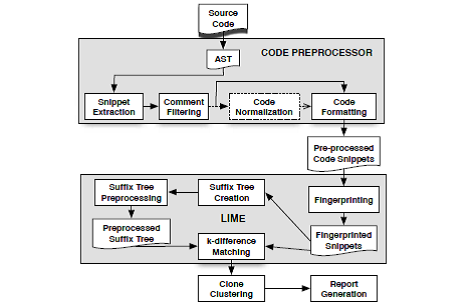
\includegraphics[width=10cm]{clone_detection}
\caption{Clone Detection Process}
    \label{fig:detect}
\end{figure}

To understand the evolution of code clone, ~\cite{empirical} developed a model of clone genealogy. In the model, 

 \begin{figure}[h]
 \centering
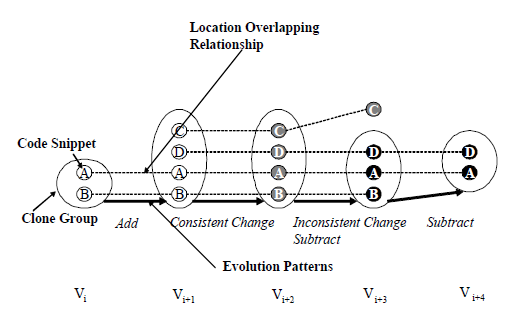
\includegraphics[width=8cm]{lineage}
\caption{An Example of Clone lineage}
    \label{fig:linea}
\end{figure}

 \begin{figure}[h]
 \centering
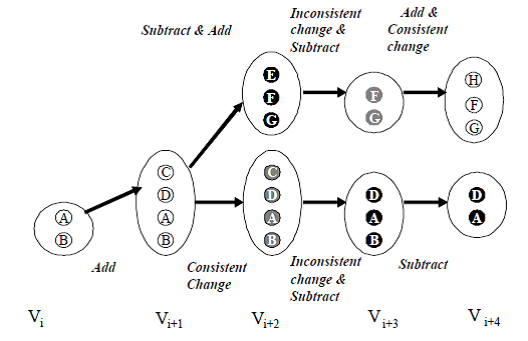
\includegraphics[width=8cm]{genealogy}
\caption{An Example of Clone Genealogy}
    \label{fig:genea}
\end{figure}

Code clone roots in the limitation of programming languages and comes out as programmers reuse pieces of code for strategies like forking, templating and customization. As long as programmers go on adopting strategies of forking to bootstrap development of similar solutions, templating for abstraction and customization for new features, code clone will remain a big issue within software development.~\cite{frontiers} For this particular reason, understanding how clones evolve, examining the cons and pros of code clone, and further more, detecting and managing clones in code will remain themes of software engineering.

\section{Project Goals}
Here we have to focus on \textit{PUGT}-Document some problem \textit{P} with some user group \textit{U} using some software tool \textit{T} to achieve some goal \textit{G}.\\
\textit{P}: Efficient copy and pasting for coders. It is focused in section \ref{Copy}.\\
\textit{U}: The target user groups are programmers specifically Java programmers.\\
\textit{G}: The goal of this project to provide features to improve copy and pasting solutions. The possible implementable featues are described in subsection $5.1$.\\
\textit{T}: The tool we will use is the Eclipse IDE.

\subsection{Project Features} 
1. Multi-item\\
 User often switches back and forth between windows to copy and paste. If we can design a clipboard that holds \textit{ multiple item at a time}, it can reduce switching. For example, if a user copies a students name, email address, institution name to a form, a multi- item clipboard manager can hold each item separately and paste it altogether.
 
 Multiple item can also be from multiple windows. Figure \ref{fig:Multi} describes two different variations of multiple item copy pasting ~\cite{cpHabits}. The upper portion is copying multiple items from a single source. The bottom portion depicts copying from multiple windows.
 
 The proposed method for copying multiple items from a single source has already been described above. For multiple items from different windows, the copied item from all the sources will be pasted to destination at a time, and each copied item from one window  will move to the next window via clipboard.
 
 \begin{figure}[h]
 \centering
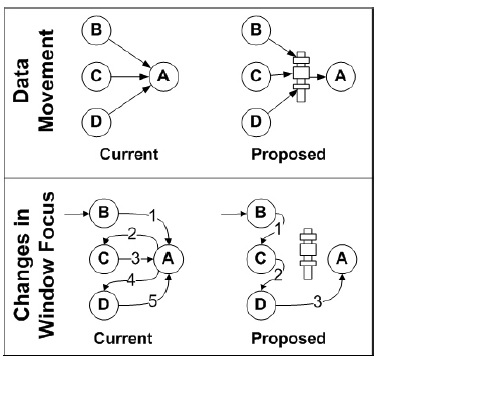
\includegraphics[width=8cm]{MultiItem}
\caption{Multiple Item Copy and Pasting}
    \label{fig:Multi}
\end{figure} 

2. System Wide copy\\
For this purpose, we perform a finer level of analysis and consider user copy and paste behavior between windows, where an application may have multiple windows (e.g., worksheets in spreadsheets, tabs in browsers,  find dialog for a word processor). A graphical representation of system wise copy and pasting is illustrated in Figure \ref{fig:System} ~\cite{cpHabits}. Advanced window management techniques such as restacking or rolling partially overlapping windows have been shown to be effective ~\cite{overlapWindow}. Adding a feature to reduce the overhead of switching among multiple windows would be desirable.

 \begin{figure}[h]
 \centering
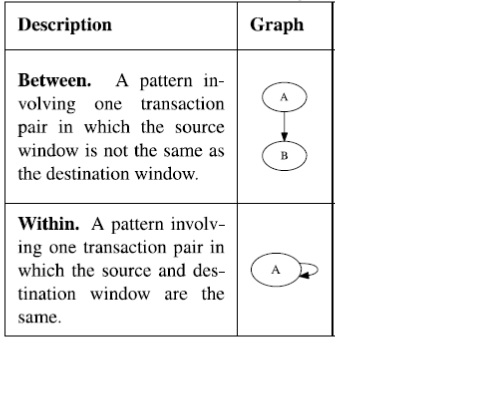
\includegraphics[width=7cm]{Window}
\caption{System Wide Copy and Pasting}
    \label{fig:System}
\end{figure} 

3. Context Awareness\\
If a user has to switch between windows to copy and paste, a context aware clipboard can reduce many transitions by allowing multiple related copies or pasting. Two parts or points have to be considered for context awaring copy and pasting:\\
    a. How do we order the items based on contextual information?\\
    b. How do we paste items ?
    
    Some clipboards like Citrine ~\cite{Citrine} and Entity Quick Click ~\cite{Entity} support context awareness features partially. Citrine is an intelligent clipboard: it copies data, extracts contextual information and partition the data accordingly. Thus ordering of items are done. Regarding the second part, Citrine allows user to paste all the partitioned data to the destination in a single click. But the user is responsible for manipulating Citrine to map the data for pasting. Entity works in a similar fashion like Citrine. Item ordering of Entity allows user to select multiple items with a single click on each item, gathers contextual information, and partitions data accordingly. For pasting, user is responsible for integrating contextual support and multiple pasting.

4. Code Cloning\\
 If developers modify a code fragment, they have to determine
whether or not to modify its code clones in source code. An intelligent clipboard can  give some suggestions to manage code cloning more smartly. Possible features could be-detect code cloning, and displaying message - "You copied here, forgot to get change here." There are tools for code clone detection,  ~\cite{CloneTag}, we could incorporate these idea into clipboards.

5. Design Pattern detection\\ 
Design patterns are typically used as guidelines during
software development.Recovering design patterns can enhance existing source code analysis tools by bringing program understanding to
the design level. The paper ~\cite{Pattern} discusses the state-of-the-art pattern detection tools.It would be really beneficial to software developers if we could identify whether code pasted follows the recommended  design patterns.

6. Touch Screen Interactions\\
If there is touch screen environment support, features could be included such as :tap on code fragments to be copied, and paste at desired destination. \\
7. Intelligent Display Manager\\
~\cite{bworld}

\section{Conclusion}
All programmers make use of the copy-paste functionality as part of their work-flow while programming. Studies have shown that the average programmer performs these actions 16 times in an hour, and uses the default system clipboard for this. Using the default system clipboard can lead to a few unintended consequences such as code cloning, issues with using common design patterns, and a general reduction in productivity by having to switch between files, projects, and windows while copy-pasting code multiple times.

While there are a several clipboard managers that deal with some of these problems, not many of them are targeted specifically at programmers, or implement features to tackle all of these problems.

We propose Clipit, an intelligent Eclipse clipboard extension that is designed specifically to improve a programmers productivity, and make programming better. Clipit has features such as being multi-item, reducing the time taken while pasting a previously copied item by eliminating the time taken to switch between windows. It also orders items and displays code intelligently, knowing when to show only a portion of a large chunk of code. Clipit also uses keyboard shortcuts similar to those used the default clipboard manager, making it easy to use. 

\bibliographystyle{abbrv}
\bibliography{citations}

%\balancecolumns 

\end{document}